\section{Zielsetzung}
In diesem Versuch wird die effektive Masse der Leitungselektronen in n-dotiertem GaAs bestimmt.
Dazu wird die Faraday-Rotation zweier n-dotierter GaAs Proben und einer reinen GaAs Probe vermessen.

\section{Theorie}
\subsection{Bandstruktur und effektive Masse}

Die Bandstruktur ist in der Festkörperphysik ein zentrales Element, um die Eigenschaften
eines Festkörpers zu beschreiben. Mit diesem Konzept können beispielsweise elektrische, thermische
und optische Eigenschaften eines Materials beschrieben werden. Außerdem lassen sich Größen wie die
effektive Masse und die Zustandsdichte beschreiben.

Die Bandstruktur für Halbleiter weißt zwischen dem Valenzband und dem Leitungsband typischerweise
eine Energielücke von $\SI{0,1}{}$ bis $\SI{4}{\eV}$ auf. Durch Dotierung eines Halbleiters
verändert sich das Bändermodell, indem Niveaus innerhalb der Bandlücke entstehen.
Für n-dotierte Halbleiter wird durch dieses zusätzliche Niveau die Bandlücke verkleinert.

\begin{figure}[H]
  \centering
  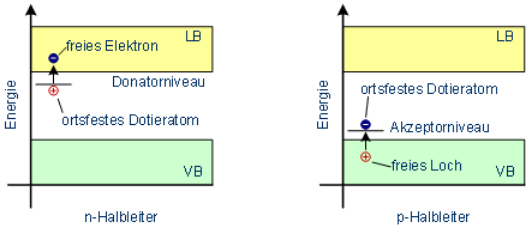
\includegraphics[width=10cm]{Bandstruktur.png}
  \caption{Bändermodell dotierter Halbleiter \cite{halbleiter}.}
  \label{fig:Band}
\end{figure}

Zur Weiteren Beschreibung von Festkörpern wird häufig die effektive Masse verwendet.
Für freie Elektronen gilt eine quadratische Dispersionsrelation
\begin{equation}
  E(\vec{k})=\frac{\hbar^2 \vec{k}^2}{2m}
\end{equation}
mit der Elektronenmasse $m$ und dem Wellenvektor $\vec{k}$.

Für Kristallelektronen, welche gebunden sind und sich im Potential der
Atomkerne befinden, gilt diese Dispersionsrelation nicht. Für gebundene
Elektronen tritt pro Atom nur eine effektive Anzahl von Elektronen mit der einfallenden
Strahlung in Wechselwirkung. Da nur diese effektiven Elektronen die optischen
Eigenschaften des Festkörpers bestimmen, werden sie auch als Dispersionselektronen
bezeichnet. Analog zur Anzahl der effektiven Elektronen lässt sich auch eine
effektive Masse $m^*$ bestimmen. Aus der Bandstruktur kann diese über die Krümmung des
Leitungsbandes am Punkt $\vec{k}=\vec{0}$ nach

\begin{equation}
  m^*_i=\hbar^2\Big(\frac{\partial^2 E}{\partial k^2_i} \Big)^{-1}
\end{equation}
bestimmt werden. Diese Größe $m^*_i$ ist dabei richtungsabhägig. Bei ausreichender
Kristallsymmetrie kann sie jedoch als isotrop angenommen werden und zur richtungsunabhängigen
Größe $m^*$ vereinfacht werden. Für GaAs liegt diese außreichende Kristallsymmetrie vor und es kann
die Größe $m^*$ verwendet werden.

Unter Verwendung der effektiven Masse $m^*$ kann wieder die Quantenmechanik eines
freien Teilchens angenommen werden, da das Potential schon in der effektiven Masse
berücksichtigt ist.

\subsection{Doppelbrechung}
Das Phänomen der Doppelbrechung bezeichnet die Eigenschaft optisch anisotroper Medien einen Lichtstrahl in
zwei senkrecht zueinander polarisierte Teilstrahlen aufzuspalten. Dieser Effekt ist bei allen Kristallen, außer
denen des kubischen Kristallsystems, zu beobachten. Ein bekanntes Beispiel für einen doppelbrechenden Kristall ist
Kalkspat.
Fällt unpolarisiertes Licht auf einen doppelbrechenden Kristall, so wird der
Lichtstrahl in zwei Teilstrahlen aufgespalten. Der ordentliche Strahl (o-Strahl)
verhält sich nach dem Snellius'schen Brechungsgesetz, während der außerordentliche Strahl
(ao-Strahl) nicht diesem Gesetz folgt. Dies ist für den Fall eines senkrecht
einfallenden Lichtstrahls in Abbildung \ref{fig:Doppelbrechend} dargestellt.

\begin{figure}[H]
  \centering
  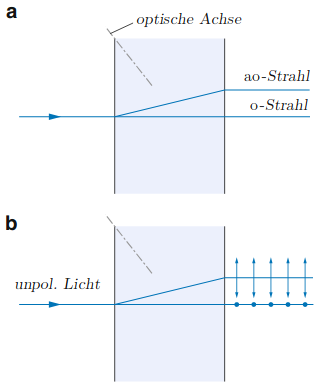
\includegraphics[height=7cm]{Doppelbrechend.png}
  \caption{Schematische Darstellung eines doppelbrechenden Kristalls mit ordentlichem und außerordentlichem Strahl \cite{Heintze}.}
  \label{fig:Doppelbrechend}
\end{figure}

Der ao-Strahl liegt dabei immer in der Ebene, welche den o-Strahl und die
optische Achse enthält. Außerdem sind beide Strahlen linear polarisiert.
Für den o-Strahl liegt die Polarisation senkrecht zu der Ebene, welche den o-Strahl und die
optische Achse enthält. Die Polarisation des ao-Strahls liegt genau in dieser Ebene.
Für den Fall, dass das einfallende Licht schon in eine dieser Richtungen polarisiert ist
kommt es nicht zur Doppelbrechung und es gibt nur einen Strahl.
Ein Weiterer Sonderfall ist der Lichteinfall parallel zur optischen Achse, denn dann
kommt es ebenfalls nicht zur Doppelbrechung und es gibt nur einen Strahl.


Fällt nun jedoch linear polarisiertes Licht in Richtung der optischen Achse ein, so kommt es
bei optisch anisotropen Kristallen zur Drehung der Polarisationsrichtung. Dieses Phänomen wird
auch als optische Aktivität bezeichnet und lässt sich mithilfe der zirkularen Doppelbrechung
beschreiben.
Linear polariesiertes Licht kann als Überlagerung von links- und rechtszirkular
polarisiertem Licht aufgefasst werden. Durchläuft dieses Licht einen doppelbrechenden Kristall, kommt
es aufgrund der optischen Anisotropie zu unterschiedlichen Phasengeschwindigkeiten für die beiden zirkular
Polarisierten Strahlen und damit auch zu einer Phasenverschiebung. Dies führt
zu einer Drehung der Polarisation um den Winkel

\begin{equation}
  \theta=\frac{L}{2}(k_R -k_L).
\end{equation}
Dabei bezeichnet $L$ die Länge des Kristalls und $k_i$ den jeweiligen Wellenvektor.



\subsection{Induzierte Doppelbrechung-Faraday Effekt}
In optisch inaktiven Medien, welche nicht doppelbrechend sind, kann durch Anlegen eines Magnetfeldes in Ausbreitungsrichtung des Lichts
Doppelbrechung hervorgerufen werden. Das Magnetfeld induziert in den Atomen zusätzliche Kreisströme, wodurch es zu einer Asymmetrie im
Kristall kommt, welche zu unterschiedlichen Brechungsindizes für links- und rechtspolarisiertes Licht führt. Dies hat zur Folge, dass es
bei dem Einfall von linear polarisiertem Licht, welches parallel zum Magnetfeld in den Kristall einfällt zu einer Drehung der
Polarisationsebene kommt. Dieser Effekt wird auch als Faraday-Effekt bezeichnet.
Der Drehwinkel $\theta$ ist dabei von der Stärke und Richtung des Magnetfeldes abhängig sowie von der Länge $l$ des Kristalls:
\begin{equation}
  \theta=VBL.
\end{equation}
Die Verdet-Konstante $V$ ist dabei eine für den Stoff charakteristische Größe und ist stark von der Wellenlänge abhängig.

Aus der Bewegungsgleichung für ein gebundenes Elektron sowie den Polarisationseffekten im Kristall lässt sich folgende Gleichung
für den Drehwinkel $\theta$ aufstellen:

\begin{equation}
  \theta(\lambda)=\frac{2\pi^2e_0^3c}{\epsilon_0 m^2 \lambda^2 \omega_0^4}\cdot\frac{NBL}{n}
\end{equation}
Diese Relation bezieht sich auf alle Ladungsträger im Kristall, sowohl die gebundenen Kristallelektronen, als auch die
freien Elektronen durch die Dotierung.

Die Rotation der freien Elektronen kann anhand der Gleichung
\begin{equation}
  \theta_\text{frei}(\lambda)=\frac{e_0^3}{8\pi^2\epsilon_0c^3(m*)^2}\cdot\lambda^2\cdot\frac{NBL}{n}
\end{equation}
bestimmt werden.
